\section{The look-ahead tails in full}
\label{app:tails}

This appendix documents the audit behind \S\ref{sec:mechanism}: what a $K{=}5$ tail is, how
often it is cut short and why, what the oracle does with it, and what it costs in API calls.
All scores are the training oracle's, read from the per-candidate training logs of the two
\Kf{} arms ($59{,}868$ PTO and $55{,}552$ GRPO candidates); GRPO \Kf{} is right-censored at
iteration~5, and its iterations 1--2 are partial logs (a crash-and-resume kept only the
post-resume steps: log coverage $0.50$ / $0.71$), so those rows describe the later part of
the iteration.

\paragraph{What a tail is, and the ``patient closed'' fingerprint.} A tail is the
oracle-format transcript slice appended to the candidate --- patient reply, then up to four
more alternating turns generated by the same policy and simulator --- so a full tail has five
turns and the number of realized turns is the number of role labels in it (0 mismatches over
$115$k tails). The simulator ends a session by writing a \texttt{SESSION ENDED} marker; the
look-ahead code strips that marker and keeps only the text before it, so the marker itself
appears in $0$ tails. What survives is a trailing whitespace on the last patient turn. We
validated this fingerprint two ways. In the evaluation conversations, where the end reason
is recorded, $398/398$ patient-closed rows end in whitespace against $279/7{,}306 = 3.8\%$
of ordinary patient rows. In the tails, the last patient turn carries a wrap-up phrase
(``wrap'', ``for now'', ``next time'', ``thank \ldots'') in $89.7\%$ (PTO) / $87.6\%$
(GRPO) of fingerprinted patient-closed tails against $24.8\%$ / $11.9\%$ of full open tails.
We treat the patient-closed shares as accurate to $\pm 2$--$4$ percentage points; odd-length
tails without the fingerprint are labelled therapist-stalled and are the fingerprint's
complement.

\begin{table}[t]
  \centering\footnotesize
  \setlength{\tabcolsep}{3pt}
  \begin{tabular}{@{}lrrrrrrr@{}}
    \toprule
    arm & iter & cand. & ended & patient & no & ther. & loop \\
        &      &       & early & closed  & tail & end  &  \\
    \midrule
    PTO \Kf{}  & 1  & 7,097 & .210 & .191 & .007 & .011 & .088 \\
               & 2  & 6,685 & .204 & .190 & .002 & .009 & .060 \\
               & 3  & 6,522 & .220 & .205 & .004 & .010 & .051 \\
               & 4  & 4,899 & .265 & .254 & .004 & .006 & .012 \\
               & 5  & 3,351 & .354 & .286 & .028 & .039 & .007 \\
               & 6  & 5,289 & .264 & .255 & .001 & .005 & .004 \\
               & 7  & 6,444 & .249 & .234 & .004 & .009 & .004 \\
               & 8  & 6,117 & .213 & .194 & .004 & .012 & .002 \\
               & 9  & 6,077 & .206 & .192 & .003 & .010 & .000 \\
               & 10 & 7,387 & .182 & .167 & .003 & .008 & .000 \\
               & all & 59,868 & .228 & .211 & .005 & .011 & .025 \\
    \midrule
    GRPO \Kf{} & 1  & 6,912 & .169 & .113 & .037 & .018 & .279 \\
               & 2  & 9,472 & .173 & .124 & .030 & .019 & .178 \\
               & 3  & 14,336 & .158 & .124 & .023 & .011 & .072 \\
               & 4  & 13,568 & .204 & .188 & .013 & .003 & .007 \\
               & 5  & 11,264 & .252 & .235 & .015 & .002 & .002 \\
               & all & 55,552 & .192 & .161 & .022 & .009 & .086 \\
    \bottomrule
  \end{tabular}
  \caption{Tail structure by training iteration (share of candidates). \emph{ended early}
    $=$ fewer than five realized turns; \emph{patient closed} $=$ fingerprinted session end;
    \emph{no tail} $=$ zero simulated turns; \emph{ther.\ end} $=$ tail ends on a therapist
    turn; \emph{loop} $=$ a therapist turn in the tail verbatim-repeats the candidate or
    another tail turn. Therapist-stalled tails are $\leq 0.5\%$ in every row ($0.2\%$ PTO /
    $0.05\%$ GRPO pooled) and omitted. A
    further $13.5\%$ (PTO) / $9.8\%$ (GRPO) of candidates have a full five-turn tail whose
    fifth (patient) turn closes the session. Bootstrap CIs on the ended-early rate are
    $\pm 0.003$--$0.017$ per row (Table \texttt{tail\_audit\_by\_iter}).}
  \label{tab:tail_by_iter}
\end{table}

\paragraph{How often, and why, tails end early.} Table~\ref{tab:tail_by_iter}. The rate is
not flat: it peaks at iteration~5 in both arms ($0.354$ PTO, $0.252$ GRPO) and then falls in
PTO to $0.182$ by iteration~10. Iteration~5 of PTO \Kf{} is also an infrastructure incident
(below), which accounts for part of that spike ($0.028$ no-tail plus $0.039$
therapist-end) though patient closes rise as well ($0.286$). Degeneration inside tails is
confined to early iterations: verbatim loops fall from $27.9\%$ of GRPO tails at iteration~1
to $0.2\%$ at iteration~5; no ChatML role-marker leaks occur in any tail; candidates
floored to reward $0$ are $\leq 0.2\%$.

\begin{table}[t]
  \centering\scriptsize
  \setlength{\tabcolsep}{2pt}
  \begin{tabular}{@{}lrrrrrr@{}}
    \toprule
    arm & iter & $\Delta$(ee$-$full) & \dz{} & RR & P(argmax ee) & base \\
    \midrule
    PTO \Kf{}  & 1  & $-0.043$ & $-0.24$ & 0.77 & .170 & .210 \\
               & 3  & $-0.042$ & $-0.26$ & 0.79 & .183 & .220 \\
               & 5  & $-0.034$ & $-0.21$ & 0.82 & .310 & .354 \\
               & 7  & $-0.034$ & $-0.27$ & 0.77 & .203 & .249 \\
               & 8  & $-0.017$ & $-0.15$ & 0.69 & .158 & .213 \\
               & 10 & $-0.038$ & $-0.38$ & 0.67 & .130 & .182 \\
               & all & $-0.034$ & $-0.24$ & 0.77 [0.74, 0.80] & .186 & .228 \\
    \midrule
    GRPO \Kf{} & 1  & $-0.094$ & $-0.32$ & 0.71 & .126 & .169 \\
               & 3  & $-0.073$ & $-0.33$ & 0.74 & .122 & .158 \\
               & 4  & $-0.015$ & $-0.10$ & 0.83 & .176 & .204 \\
               & 5  & $-0.037$ & $-0.28$ & 0.80 & .212 & .252 \\
               & all & $-0.051$ & $-0.26$ & 0.79 [0.75, 0.82] & .158 & .192 \\
    \bottomrule
  \end{tabular}
  \caption{Within-group effect of the tail ending (training oracle). $\Delta$(ee$-$full)
    $=$ mean score of ended-early candidates minus mean score of full-tail siblings, paired
    within groups holding both kinds (\QQ{} points; PTO $3{,}809$ groups pooled, GRPO
    $2{,}878$); every per-iteration row is Holm-significant within arm ($p_{\text{Holm}}
    \leq .004$). RR $=$ P(argmax $\mid$ ended early) $/$ P(argmax $\mid$ full); P(argmax
    ee) $=$ share of groups whose winner ended early, against the base rate of ended-early
    candidates. Group-bootstrap 95\% CIs on the pooled RR in brackets.}
  \label{tab:tail_within}
\end{table}

\paragraph{What the oracle does with the ending.} Table~\ref{tab:tail_within}. Within a
group, ended-early siblings score lower than full-tail siblings by $0.03$--$0.05$ points and
are chosen as the argmax about $23\%$ less often; the disfavour grows over PTO training. By
realized length (pooled), the score deviation from the group mean is $-0.067$ / $-0.071$
(PTO / GRPO) for no tail, $-0.012$ / $-0.009$ for one turn (patient closes at once),
$-0.064$ / $-0.071$ for two, $-0.005$ / $-0.001$ for three, $-0.079$ / $-0.110$ for four,
and $+0.004$ / $+0.004$ for a full tail; P(argmax) is $0.04$--$0.10$ on the even lengths and
$0.10$--$0.13$ on the odd ones and full tails. The penalty is therefore concentrated on the
$2$--$3\%$ of failure tails, not on the patient closing. These are within-group
associations: a candidate that makes the patient close and a shorter transcript for the
oracle are confounded, and raw (between-group) scores of patient-closed tails are
\emph{higher} than full tails because they occur late in high-scoring conversations.

\paragraph{The tail mirrors the candidate.} Pooled lexical cues in the tail's therapist
turns against the scored candidate: questions per turn $0.42$ vs.\ $0.45$ (PTO), $0.70$ vs.\
$0.66$ (GRPO); affirmation regex rate $0.058$ vs.\ $0.068$ / $0.031$ vs.\ $0.041$; effusive
praise $0.040$ vs.\ $0.030$ / $0.006$ vs.\ $0.006$. Across PTO \Kf{} training the candidate
length triples ($307 \to 1{,}006$ chars, iterations 1 to 10) while questions per turn halve
($0.61 \to 0.27$) and effusive praise rises ($0.004 \to 0.078$); GRPO \Kf{} candidates go
$324 \to 585$ chars over iterations 1--5.

\begin{figure}[t]
  \centering
  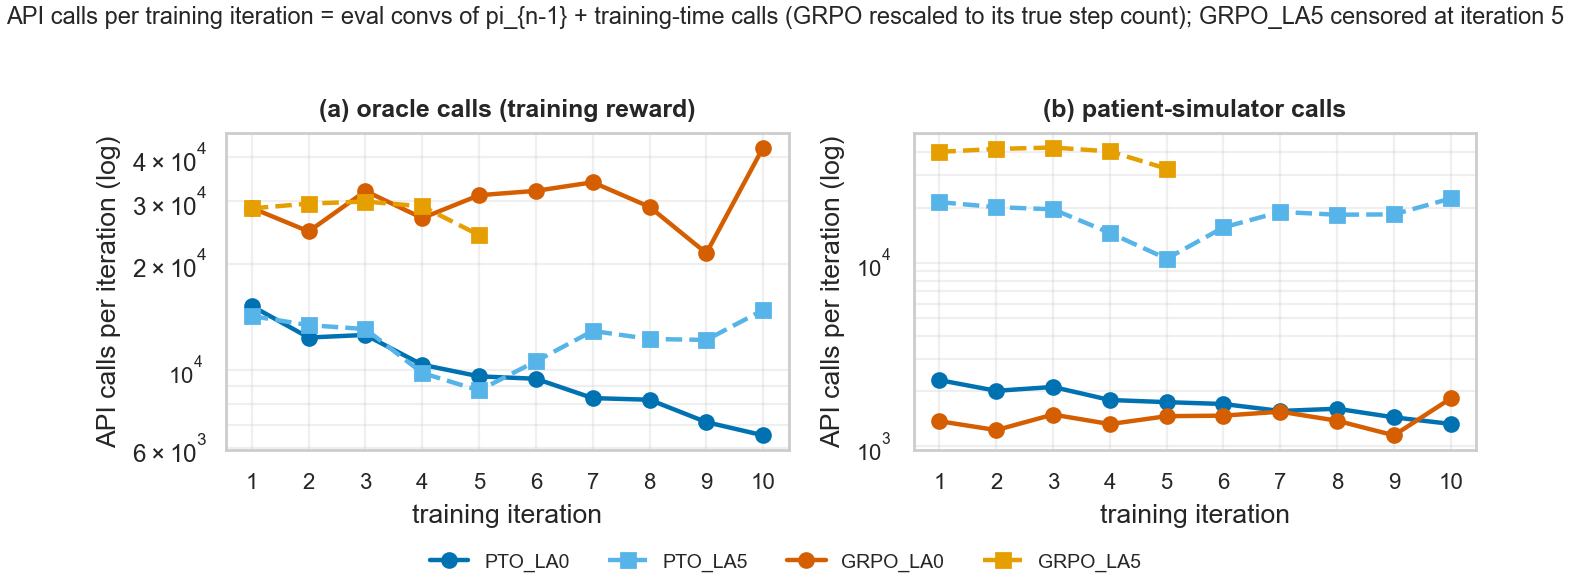
\includegraphics[width=\linewidth]{figures/tail_audit_fig_api.png}
  \caption{API calls per training iteration by arm (log scale): (a) oracle calls, (b)
    patient-simulator calls. GRPO calls are rescaled to the true optimizer-step count where
    the log is partial. GRPO \Kf{} is censored at iteration~5.}
  \label{fig:api}
\end{figure}

\begin{table}[t]
  \centering\scriptsize
  \setlength{\tabcolsep}{2pt}
  \begin{tabular}{@{}lrrrrr@{}}
    \toprule
    & iters & oracle calls & oracle Mchars & patient calls & total \\
    \midrule
    PTO \Kz{}   & 1--5  & 59,991  & 516.2   & 9,950   & 69,941 \\
    PTO \Kf{}   & 1--5  & 59,177  & 622.2   & 86,114  & 145,291 \\
    \quad ratio &       & 0.986   & 1.205   & 8.655   & 2.077 \\
    PTO \Kz{}   & 1--10 & 99,622  & 987.1   & 17,587  & 117,209 \\
    PTO \Kf{}   & 1--10 & 121,806 & 1,849.2 & 179,634 & 301,440 \\
    \quad ratio &       & 1.223   & 1.873   & 10.214  & 2.572 \\
    GRPO \Kz{}  & 1--5  & 143,548 & 1,117.4 & 6,879   & 150,427 \\
    GRPO \Kf{}  & 1--5  & 141,237 & 1,519.8 & 197,239 & 338,476 \\
    \quad ratio &       & 0.984   & 1.360   & 28.673  & 2.250 \\
    \bottomrule
  \end{tabular}
  \caption{Training-time API calls summed over matched iterations (Table
    \texttt{tail\_audit\_api\_ratio}). Oracle calls $=$ 2 per scored candidate plus logged
    retries; Mchars $=$ millions of characters the oracle read (prefix, completion, tail,
    two rubrics; the $\sim$1k-token cached rubric prefix excluded); patient calls $=$
    eval-conversation turns $+$ PTO trunk replies $+$ realized patient turns inside tails
    ($2.65$ per candidate for PTO, $2.87$ for GRPO). Run-Eval scoring adds $96 \times 8 =
    768$ calls per model state per grader, identical across arms.}
  \label{tab:api}
\end{table}

\paragraph{API cost.} Table~\ref{tab:api} and Figure~\ref{fig:api}. Oracle calls per
candidate are matched by construction ($\Kf{}/\Kz{}$ ratio $0.98$--$0.99$ over the matched
window; the ratio is not exactly $1$ because the number of branch points per iteration
follows the policy's conversation length), so the extra oracle spend is only the longer
transcript ($1.2$--$1.4\times$ characters). The multiplier is the patient simulator: $2.6$--$2.9$
calls per candidate inside tails, $8.7\times$ (PTO) and $28.7\times$ (GRPO) the \Kz{} patient
volume, so total API calls roughly double at matched iterations ($2.08\times$ PTO,
$2.25\times$ GRPO over iterations 1--5; $2.57\times$ PTO over 1--10) --- to be read beside the
$\sim$1.9$\times$ per-step GPU multiplier of \S\ref{sec:cost}. Whole-run totals: GRPO \Kz{}
(10 iterations) $302{,}541$ oracle $+$ $15{,}449$ patient calls; GRPO \Kf{} (5) $141{,}237 +
198{,}320$; PTO \Kz{} (10) $99{,}622 + 18{,}562$; PTO \Kf{} (10) $121{,}806 + 181{,}008$.

\paragraph{The PTO \Kf{} iteration-5 incident.} Iteration~5 of PTO \Kf{} logged $1{,}654$
oracle retries against $0$--$15$ in every other PTO iteration, $389$ candidates with a tail
but no score (dropped from training and from the audit), $148$ zero-turn tails among its
$3{,}740$ simulated candidates ($95$, i.e.\ $2.8\%$, among the $3{,}351$ scored ones), and only
$468$ branch points (its neighbours built $613$ and $663$); $24.8\%$ of its groups
held an unscored candidate and one group was dropped for having fewer than two valid
scores. We attribute this to a transient oracle/patient API failure. Its effect on the arm
is a smaller DPO update at that iteration, not a change to the arm's data-generating rule;
it is visible as the iteration-5 spike in Table~\ref{tab:tail_by_iter} and
Figure~\ref{fig:tails}a, and the compute axis of \S\ref{sec:cost} bills the iteration at
its measured wall-clock. Iteration~5 of GRPO \Kf{} shows a milder ended-early rise ($0.252$)
without retries.

\paragraph{Supplementary figures referenced from \S\ref{sec:behaviour}--\ref{sec:mechanism}.}
Figure~\ref{fig:shape} gives session shape by iteration, Figure~\ref{fig:wai} the WAI-SR
subscale gains at the endpoints (on the WAI-SR total, GRPO \Kf{} at iteration~5 leads \Kz{}
under the training oracle, \dz{} $-0.45$, $p_{\text{Holm}}{<}.001$, but not under the held-out
judge, \dz{} $-0.19$, n.s.), Figure~\ref{fig:composition} the per-session composition of
MI-inconsistency by iteration under both graders, Figure~\ref{fig:hetero} the $K$ contrast
within cooperation strata, Figure~\ref{fig:dispersion} the within-group dispersion of the
training reward, and Figure~\ref{fig:faithfulness} the reward-faithfulness curves. Details
behind \S\ref{sec:mechanism}: at the base policy the \Kf{}/\Kz{} margin ratio is $1.55$
[$1.46$, $1.66$] (PTO) / $1.44$ [$1.32$, $1.56$] (GRPO) and the SD ratio $1.53$ [$1.44$, $1.63$]
/ $1.40$ [$1.29$, $1.52$]; pooled over iterations the ratio of ratios is $1.02$ for both
methods. Margin/SD sits at $2.89$--$3.06$ in every arm and iteration, against $3.15$ for eight
iid normal draws and a shuffle-null range of $2.91$--$3.17$; the winner's standardized lead is
$+0.07$ SD higher under \Kf{} for PTO at the base policy and $-0.00$ [$-0.02$, $0.02$] pooled,
$+0.16$ then $+0.10$ for GRPO. The share of the pair-yield gap explained by rescaling is $0.437$
at the base policy and $0.57$ at the median over iterations 1--7, while at iterations 8--10 the
\Kf{} yield is level with (iteration~8: $0.737$ vs.\ $0.733$) or below \Kz{}'s. With the held-out judge on the evaluation side, the
matched-policy \Kz{}$-$\Kf{} faithfulness delta is $+0.007$ (PTO) / $-0.014$ (GRPO). What does
move over training is the cross-grader faithfulness of GRPO \Kz{}: it falls from $0.80$ at
iteration~1 to $0.63$ at iteration~7 ($0.70$ at iteration~10) while same-grader faithfulness
barely moves ($0.90 \to 0.85$ at iteration~7, $0.83$ at iteration~10) --- the reward keeps predicting the oracle's own verdict and stops predicting
the held-out judge's. GRPO's
length push is negative early under both $K$ ($-142$ / $-40$ chars at iteration~1) and turns
positive late. The tail's therapist turns carry the candidate's own lexical profile ($0.45$ vs.\
$0.42$ questions per turn for PTO), so the oracle scores more of the same policy plus the
patient's reaction.

\begin{figure*}[t]
  \centering
  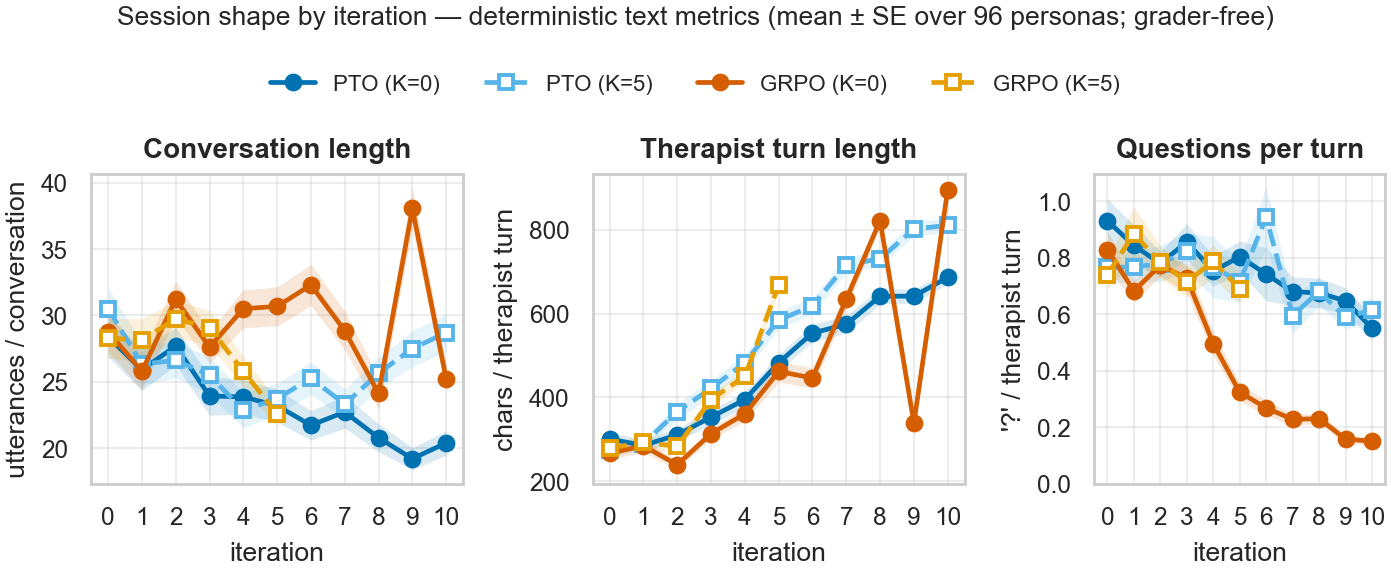
\includegraphics[width=\linewidth]{figures/session_shape_stability_fig_shape.png}
  \caption{Session shape by iteration, grader-free (mean $\pm$ SE over 96 personas), all four
    arms; GRPO \Kf{} ends at iteration~5. Look-ahead lengthens PTO sessions and shortens GRPO
    sessions; both \Kf{} arms write longer turns; GRPO \Kz{} nearly stops asking questions
    ($0.15$ per turn by iteration~10).}
  \label{fig:shape}
\end{figure*}

\begin{figure*}[t]
  \centering
  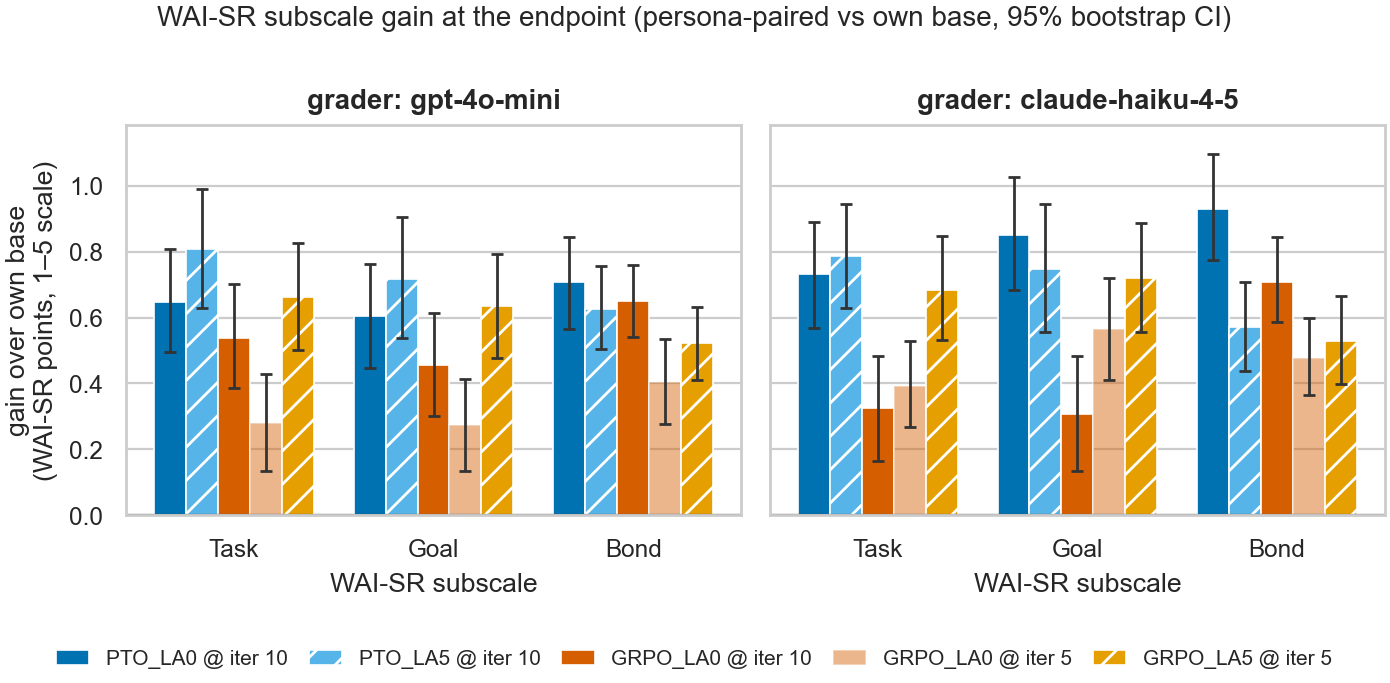
\includegraphics[width=0.8\linewidth]{figures/held_out_instruments_fig_wai.png}
  \caption{WAI-SR subscale gain over own base at the endpoints (PTO 10; GRPO 10 and, matched to
    the censored \Kf{} arm, 5), both graders. Under \Kz{} the gain is bond-weighted (except GRPO
    at iteration~5 under the held-out judge); under \Kf{} it shifts to Task and Goal,
    significantly so for PTO (Table \texttt{held\_out\_instruments\_wai\_kcontrast}).}
  \label{fig:wai}
\end{figure*}

\begin{figure*}[t]
  \centering
  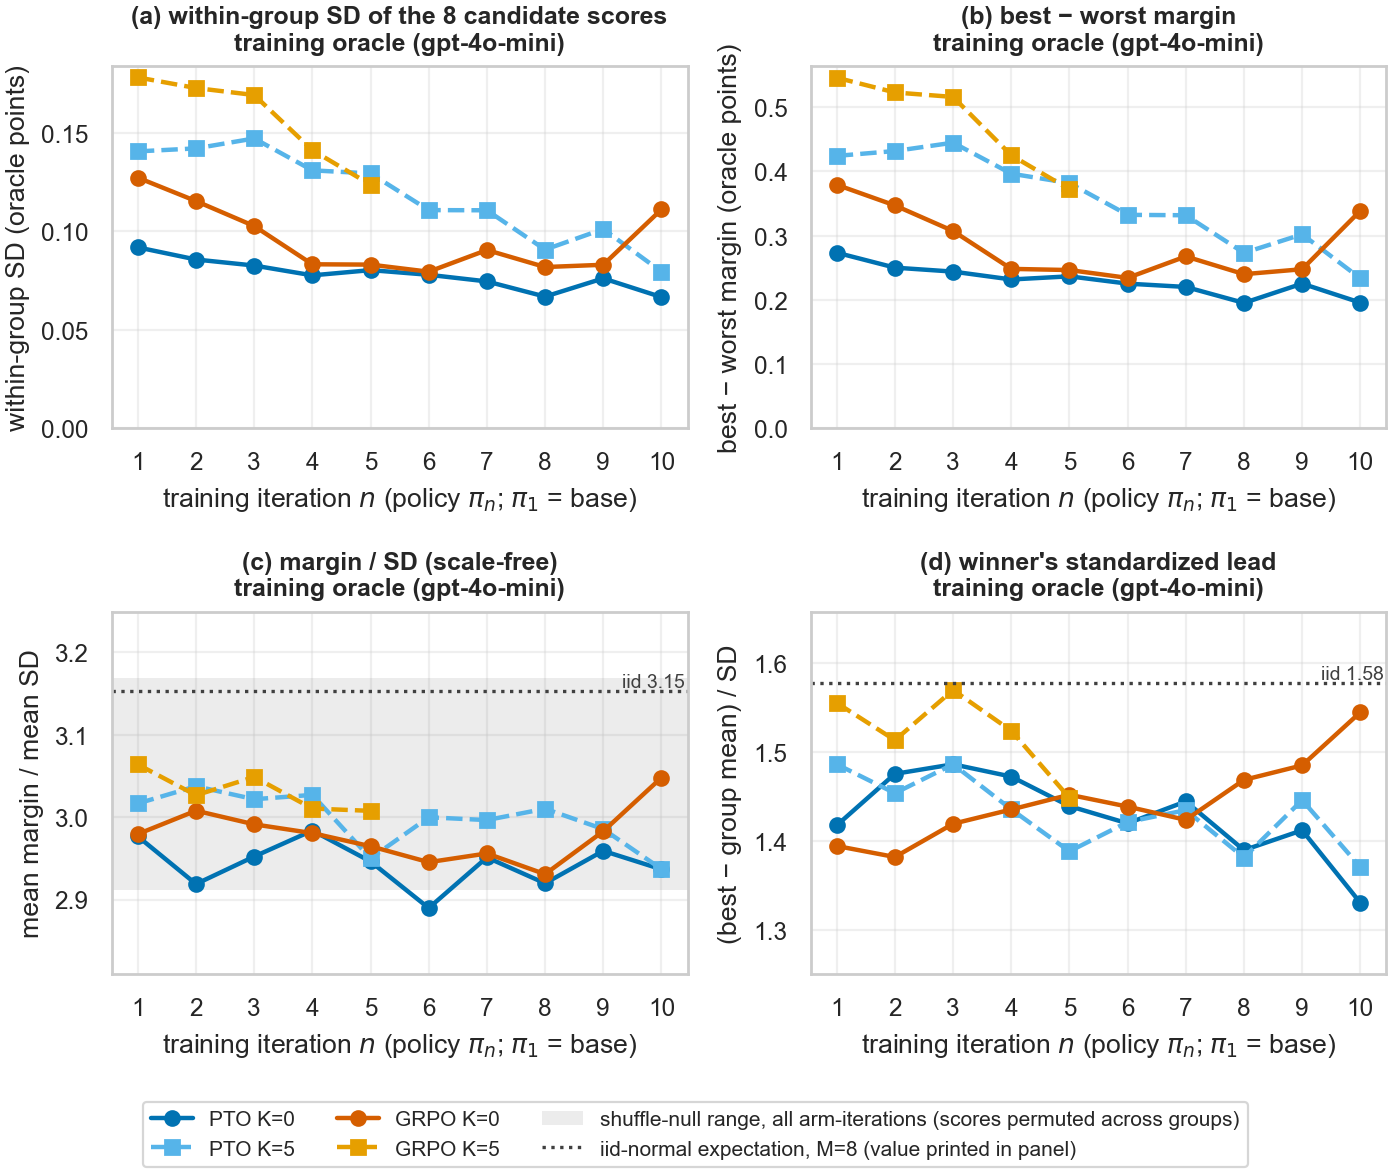
\includegraphics[width=0.85\linewidth]{figures/dispersion_by_k_fig.png}
  \caption{Within-group dispersion of the training reward over the $M{=}G{=}8$ candidates per
    branch point, by training iteration (training oracle). Look-ahead lifts both the SD (a) and
    the best--worst margin (b) by the same factor, so the scale-free statistics (c, d) stay at
    the value expected for eight exchangeable draws (dotted; grey band $=$ shuffle-null range).
    GRPO \Kf{} stops at iteration~5.}
  \label{fig:dispersion}
\end{figure*}

\begin{figure*}[t]
  \centering
  \begin{minipage}[t]{0.49\linewidth}
    \centering
    
\includegraphics[width=\linewidth]{figures/k_mici_composition_grid_gpt-4o-mini.png}
  \end{minipage}\hfill
  \begin{minipage}[t]{0.49\linewidth}
    \centering
    
\includegraphics[width=\linewidth]{figures/k_mici_composition_grid_claude-haiku-4-5.png}
  \end{minipage}
  \caption{MI-inconsistency composition in per-session counts (no turn denominator), all
    four arms by iteration, under the training oracle (left) and the held-out judge (right).
    In each grid: over-praise per session, advice-without-permission per session, all
    MI-inconsistent acts per session, and the 1--5 severity global; solid $=$ \Kz{}, dashed
    $=$ \Kf{}; GRPO \Kf{} ends at iteration~5. Over-praise collapses under \Kf{} in every arm;
    for PTO advice-without-permission rises to take its place and the per-session totals
    separate late under the training oracle but not under the held-out judge, while GRPO at
    iteration~5 is the mirror image (Table~\ref{tab:substitution}).}
  \label{fig:composition}
\end{figure*}

\begin{figure}[t]
  \centering
  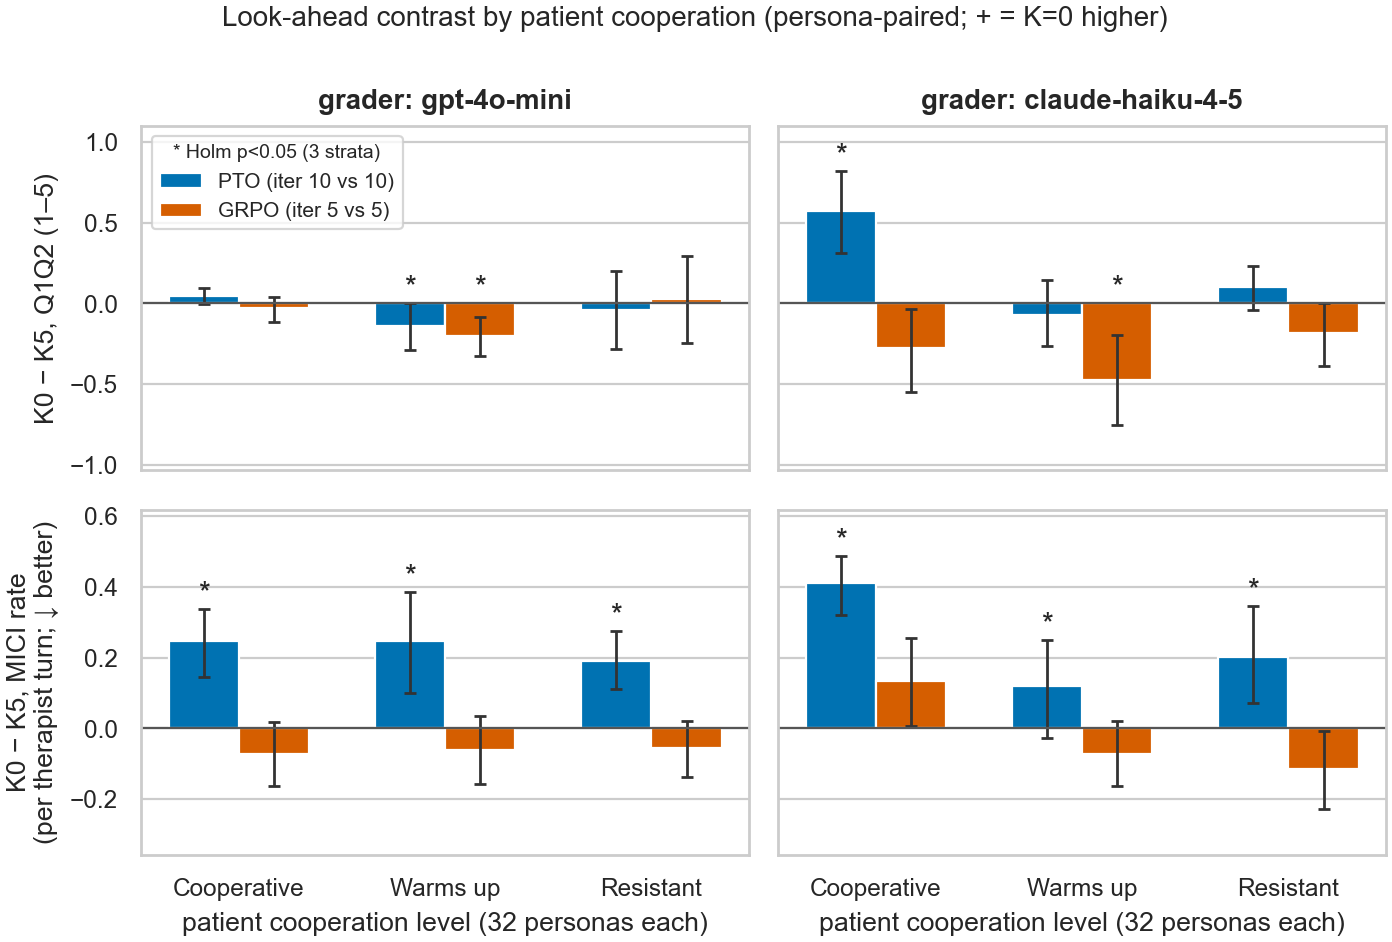
\includegraphics[width=\linewidth]{figures/held_out_instruments_fig_hetero.png}
  \caption{Persona-paired \Kz{}$-$\Kf{} within cooperation level (32 personas each) on \QQ{}
    (top) and MI-inconsistency per turn (bottom; lower is better), both graders; PTO at
    iteration~10, GRPO at its censored iteration~5; $^{*}$ Holm $p<.05$ across the three
    strata. The Cooperative stratum is at ceiling on the training oracle.}
  \label{fig:hetero}
\end{figure}

\begin{figure*}[t]
  \centering
  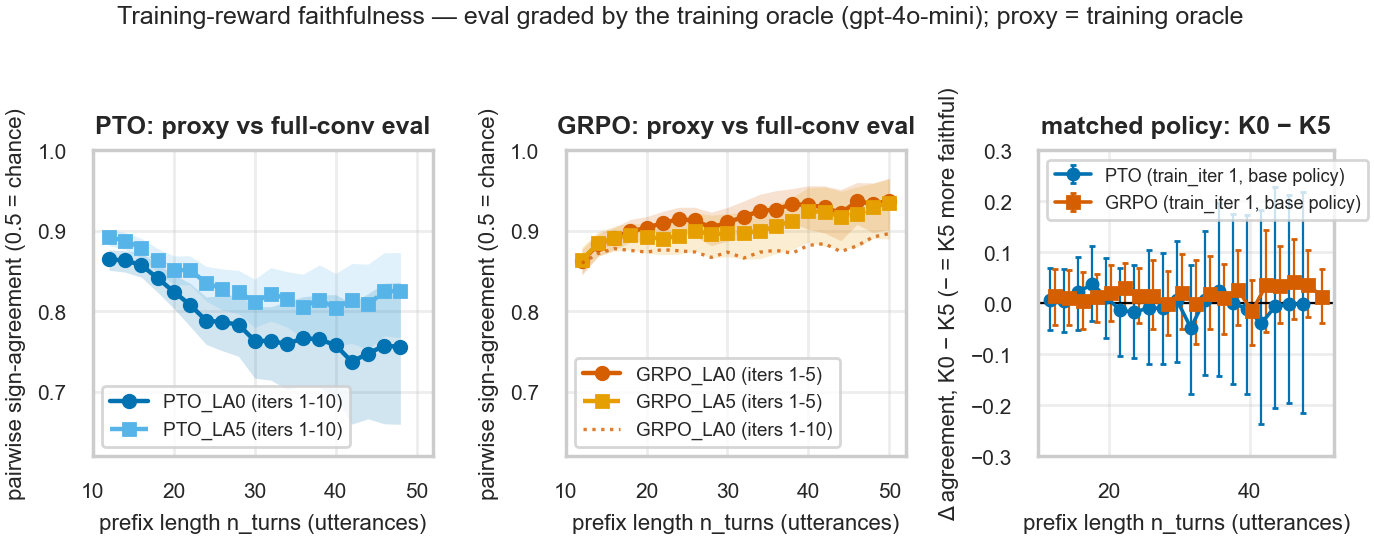
\includegraphics[width=\linewidth]{figures/reward_faithfulness_fig.png}
  \caption{Reward faithfulness: pairwise sign agreement between the training-time score of
    the chosen candidate at a prefix of $n$ utterances and the full-conversation \QQ{} of
    the evaluation conversation the prefix was cut from (training oracle on both sides;
    cluster-bootstrap ribbons). (a) PTO, (b) GRPO on its matched iterations 1--5, (c) the
    matched-policy (base) \Kz{}$-$\Kf{} delta per bin, negative $=$ look-ahead more
    faithful. The held-out-judge counterpart is \texttt{reward\_faithfulness\_fig\_heldout}.}
  \label{fig:faithfulness}
\end{figure*}
